% !Mode:: "TeX:UTF-8"
\chapter{深度学习的并行训练}

并行化和分布式计算一直是大规模机器学习中一个让人兴奋的话题, 特别是今天,越来越多的数据被应用到深度神经网络的训练中, 对训练速度提出了很高的要求。
例如,1000h的语音数据的复杂模型(LSTM, BLSTM)训练单卡需要一周左右的时间,而上万小时的数据则需迭代数月才能完成。

而深度学习依赖于大量数据,一般数据量越大,数据覆盖的范围越广,深度学习模型的效果越好。
因此,数据对于深度学习的重要性不言而喻。
海量的训练数据,对深度学习的训练速度提出了更高的要求。
在实际应用中,使用多机多卡(GPU)的解决方案加速深度学习的训练。

主流的深度学习的并行训练大致可以分为两类,基于模型的并行和基于数据的并行。
基于模型的并行,每个Worker分到模型的不同部分,仅负责对局部模型参数的更新,类似Hogwild!\ucite{recht2011hogwild}方法。
数据并行则是将数据分成多份,分别在不同Worker上处理不同的数据,适于大量数据和较小模型的训练方式。

另外一个分类方法是根据模型更新方法可以分为两类,基于梯度的模型更新和直接基于模型的更新。
基于梯度的模型更新,Server的模型更新依赖于梯度计算,如DownpourSGD\ucite{dean2012large}(既DistBelief)和ASGD。
基于模型的更新,Server和Worker的模型更新直接基于模型,通过模型之间的计算更新,如 BSP(Model Average)、EASGD和BMUF等。

本文实现基于MPI(Message Passing Interface) 的BSP、ASGD,EASGD,BMUF四种并行方法。
四种方法均是基于数据并行的方法。
BSP,EASGD和BMUF是基于模型的方法,ASGD是基于梯度的方法。
本章介绍MPI及这四种并行基本原理和实现。

\section{MPI并行计算}

MPI是一个标准化的、可移植的消息传递协议。
它由工业界和学术界联合制定,设计了一组可以在异构计算机集群上进行并行计算的接口。
并且,MPI是跨语言的通讯协议,支持多种语言用于编写并行计算机。支持点对点和广播。
MPI协议包括协议和和语义说明,指明其如何在各种实现中发挥其特性。
MPI的目标是高性能,大规模性,和可移植性。MPI在今天仍为高性能计算的主要模型。
MPI有多种实现,例如MPICH,OpenMPI\ucite{gabriel2004open}等。

深度学习的并行实现需要在多机多卡之间进行通信。
本文选用MPI作为底层通信协议,本文使用OpenMPI的MPI实现。
本文中使用的MPI的基本接口如表\ref{table:mpi}所示。

%\begin{table}
%    \begin{tabular}{ll}
%    MPI Function    & 作用                 \\
%    MPI\_Init       & MPI初始化             \\
%    MPI\_Comm\_rank & 获取MPI的rank id      \\
%    MPI\_Comm\_size & MPI节点总数            \\
%    MPI\_Allreduce  & MPI所有节点都进行reduce操作 \\
%    MPI\_Send       & MPI发送消息            \\
%    MPI\_Recv       & MPI接收消息            \\
%    \end{tabular}
%\end{table}

\begin{table}[htbp]
	\centering
	\caption{本文使用的MPI的基本接口及其作用}
	\fontsize{10.5pt}{10.5pt}\song \vspace{0.5em}
	\begin{tabularx}{\textwidth}{*2{>{\centering\arraybackslash}X}@{}}
		\toprule
    MPI Function    & 作用                 \\
		\midrule
    MPI\_Init       & MPI初始化             \\
    MPI\_Comm\_rank & 获取MPI的rank id      \\
    MPI\_Comm\_size & MPI节点总数            \\
    MPI\_Allreduce  & MPI所有节点都进行reduce操作 \\
    MPI\_Send       & MPI发送消息            \\
    MPI\_Recv       & MPI接收消息            \\
		\bottomrule
	\end{tabularx}
	\label{table:mpi}
\end{table}




\section{模型平均BSP}

BSP(Bulk Synchronize Parallel),或者称之为模型平均。
其基本思路十分简单,在训练过程中,每隔一段时间对所有Worker上的模型进行同步,
同步的模型是取所有Worker上的模型平均作为更新后的新模型。
假设$w_i$表示同步前每个Worker上的模型,
$\tilde w $表示同步后的模型,$N$为Worker总数。则:
\begin{equation}
\tilde w = \frac{1}{N}\sum\limits_{i = 1}^N {{w_i}}
\end{equation}
基于BSP的并行训练的算法描述如算法\ref{alg:bsp}所示。

\begin{algorithm}
\label{alg:bsp}
\caption{BSP模型平均}
\begin{algorithmic}
\REQUIRE 同步周期$\tau$,学习率$\eta$
%\ENSURE

\textbf{Initial:} $\tilde w$随机初始化,$t_i=0, w_i=\tilde w$,$w_i$表示第$i$个Worker上的模型。
\REPEAT
\FOR{$i\in 1,...,N$,\textbf{parallel}}
\STATE 初始化局部模型$w_i = \tilde w$
\STATE 在$\tau$更新周期内,使用本地数据, 利用SGD更新$w_i$
\STATE ${w_i} = {w_i} - \eta \nabla w_i)$, $\nabla w_i$表示Worker$i$在$t_i$时刻由训练样本的计算梯度。
\ENDFOR
\STATE 更新全局模型: $\tilde w = \frac{1}{N}\sum\limits_{i = 1}^N {{w_i}}$
\STATE ${t_i} = {t_i} + 1$
\UNTIL{(所有样本被处理完)}
\end{algorithmic}
\end{algorithm}

基于MPI的BSP算法实现如图\ref{fig:bsp}所示,使用MPI\_Allreduce函数进行Worker间的同步通信。
当到达同步周期时,所有Worker将模型从GPU卡显存复制到CPU的内存中,并除以N,
然后同时调用MPI\_Allreduce函数的SUM操作即可。

\begin{figure}[htbp]
\centering
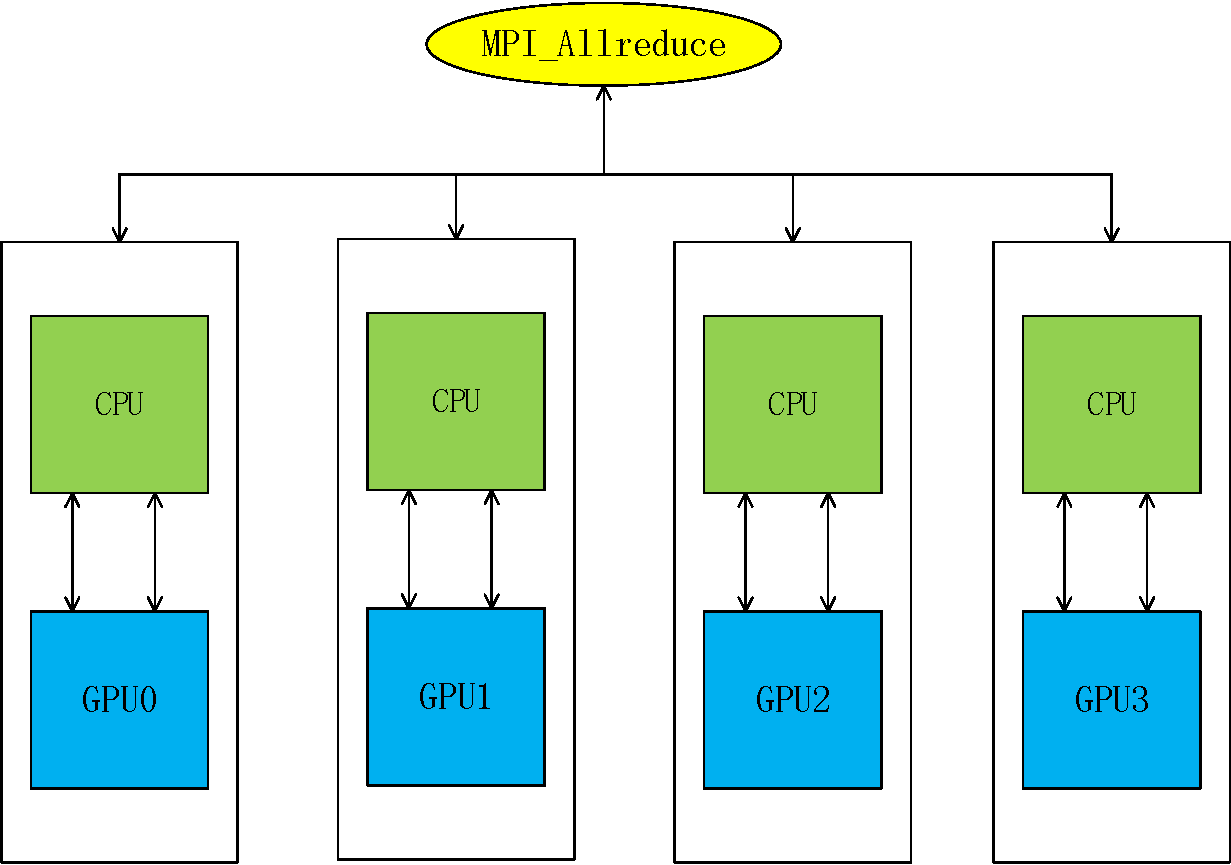
\includegraphics[width=0.5\textwidth]{figures/chapter5/bsp-crop}
\caption{基于MPI的BSP实现}
\label{fig:bsp}
\end{figure}

\section{异步随机梯度下降ASGD}

随机梯度下降SGD(Stochastic Gradient Descent)是深度学习优化的基本原理,
异步随机梯度下降ASGD(Asynchronous SGD)则是随机梯度下降的并行分布式版本。
如图\ref{fig:asgd},ASGD的深度学习系统由两部分组成:
    \begin{enumerate}
        \item 参数服务器Server,负责整体模型的存储和更新。参数服务器Server接收计算节点Worker求得的梯度,
              更新Server上的模型,并把更新后的模型发送给Worker。
        \item $N$个计算节点Worker,Worker根据本地的模型和数据计算出梯度后,将梯度发送给参数服务器,
             并从参数服务器接收最新的模型。
    \end{enumerate}

\begin{figure}[htbp]
\centering
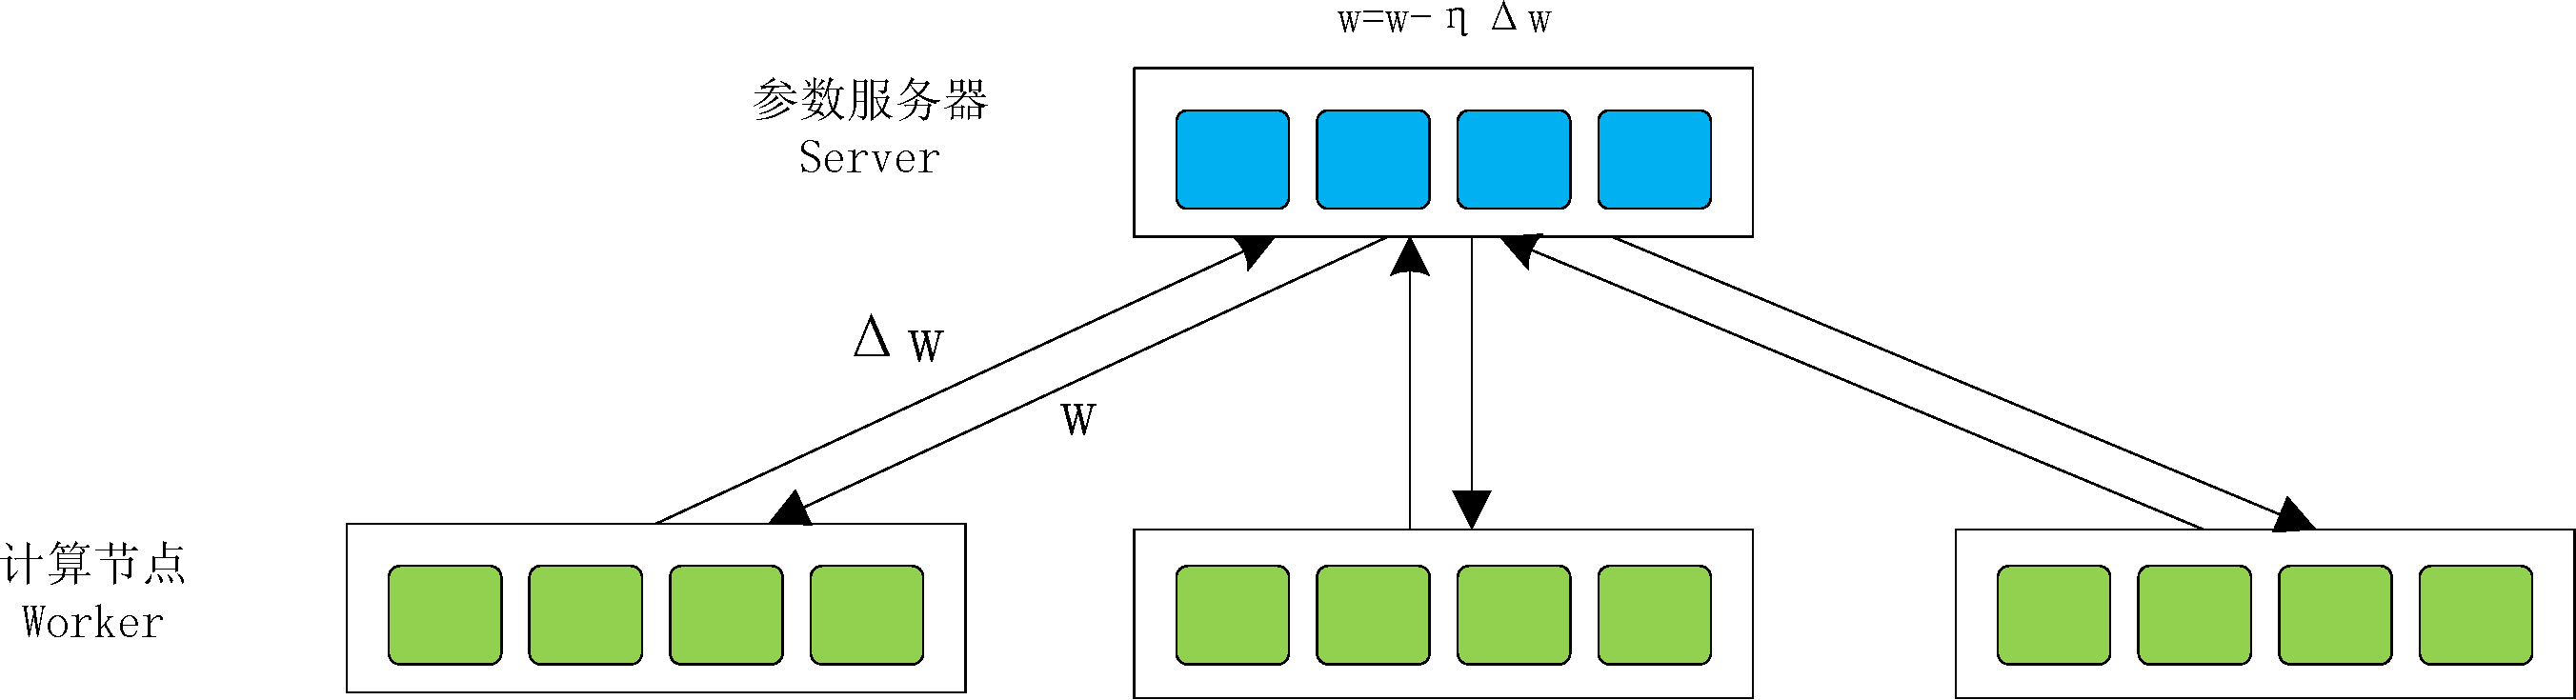
\includegraphics[width=1.0\textwidth]{figures/chapter5/asgd-crop}
\caption{异步梯度下降ASGD}
\label{fig:asgd}
\end{figure}

由图\ref{fig:asgd}可以看出,梯度是在Worker的本地模型上计算得出的梯度,
该梯度最终更新在Server的模型上,计算梯度和梯度更新的并不是同一个模型,所以
称之为异步随机梯度下降。其中Server模型的更新公式为:
\begin{equation}
{\tilde w} = {\tilde w} - \eta \nabla w_i
\end{equation}
其中$\eta$为学习率,$\nabla w_i$为当前Worker上计算发送的梯度。


在ASGD中,各个Worker独立计算,相互之间并不需要通信和同步。
每个Worker均独立和Server进行通信和模型同步,当通信和模型同步频繁时,
Server则会成为系统的性能瓶颈。
在实际应用中,同样会设定一个同步周期$\tau$,Worker计算在该周期内的累加梯度,
然后进行上述更新。$\tau$通过参数调节进行控制,$\tau$越大,Worker更新的频次越低,
系统消耗在模型等待和传输上的时间越少,系统加速的性能越好,但模型的整体效果会越差;
$\tau$越小,更新频次越高,异步程度会降低,模型效果会更好,收敛性更好,
但频繁的模型更新会导致频繁的模型同步,系统的加速性能会下降。
所以,最终同步周期$\tau$的选取则需在模型效果和加速比之间折中。

ASGD中另外一个常用的技巧是设定一个更大的全局同步周期,在该时间节点上时,
将所有Worker和Server上的模型同步为一致。
这样可以防止了各个Worker独立更新导致模型容易发散的问题,
实际应用中,我们发现采用这个技巧后模型的收敛性会更好。

\section{弹性平均随机梯度下降EASGD}

在EASGD\ucite{zhang2015deep}(Elastic Averaging SGD)中,定义优化目标为:
\begin{equation}
\label{equation:easgd}
\mathop {\min }\limits_w F(w) = \sum\limits_{i = 1}^N {f({\rm{S|}}{w_i})} {\rm{ + }}\frac{\lambda }{2}{\rm{||}}{w_i} - \tilde w|{|^2}
\end{equation}
其中$S$代表训练集,$f(.)$代表单卡的神经网络的优化目标,即训练的损失函数,可以是交叉熵CE,最小均方差MSE等的优化准则。
$\lambda$是可调的权重参数,$w_i$表示每个Worker上的模型,$\tilde w $表示Server上的模型。

所以,EASGD的优化目标为使所有Worker上的损失最小,并且各个Worker与Server之间的模型差异也要小, 这样把Worker节点上的参数跟参数服务器的中心变量联系在一起,这样使得Worker本地的模型会围绕中心Server上的模型进行变化。
上面提到,在ASGD中通过设定全局同步周期来防止各个Worker独立计算导致的模型容易发散的问题,
EASGD中则直接通过形式化的方法来达到该目标,$\frac{\lambda }{2}{\rm{||}}{w_i} - \tilde w|{|^2}$类似一个正则项,
强制Worker上的模型围绕Server上的模型进行优化。
$\lambda$比较大时,正则因子越强,Worker的模型倾向于利用当前的Server模型进行优化,
$\lambda$比较小时,正则因子越小,Worker倾向于在当前Server模型的基础上进行更多的探索。

式\ref{equation:easgd}对$\tilde w$和$w_i$进行求导有:
\begin{equation}
\begin{array}{l}
{w_i} = {w_i} - \eta \nabla {w_i} - \eta \lambda ({w_i} - \tilde w)\\
\tilde w = \tilde w - \eta \lambda \sum\limits_{i = 1}^N ( \tilde w - {w_i})
\end{array}
\end{equation}
这是同步的EASGD的更新公式。

在异步的EASGD中,略去Worker自身局部梯度$\nabla {w_i}$,略去同步,令$\alpha  = \eta \lambda$,
则单个Worker对Server模型的更新公式为:
\begin{equation}
\begin{array}{l}
{w_i} = {w_i} - \alpha ({w_i} - \tilde w)\\
\tilde w = \tilde w - \alpha (\tilde w - {w_i})
\end{array}
\end{equation}
$\alpha$控制模型的更新步长。

本文实现并使用异步的EASGD,该算法描述如算法\ref{alg:easgd}所示:
\begin{algorithm}
\label{alg:easgd}
\caption{异步EASGD}
\begin{algorithmic}
\REQUIRE 同步周期$\tau$,学习率$\alpha$ \\
%\ENSURE
\textbf{Initial:} $\tilde w$随机初始化,$t_i=0, w_i=\tilde w$,$w_i$表示第$i$个Worker上的模型。
\REPEAT
\STATE 训练数据样本$s$
\STATE $w=w_i$(中间变量)
\IF{($\tau$整除$t_i$)}
\STATE ${w_i} = {w_i} - \alpha ({w} - \tilde w)$
\STATE $\tilde w = \tilde w - \alpha (\tilde w - {w})$
\ENDIF
\STATE ${w_i} = {w_i} - \eta \nabla w_i(s)$, $\nabla w_i(s)$表示Worker$i$在$t_i$时刻由样本$s$的计算梯度。
\STATE ${t_i} = {t_i} + 1$
\UNTIL{(所有样本被处理完)}
\end{algorithmic}
\end{algorithm}

\section{BMUF}

2016年,微软在语音识别任务上提出BMUF\ucite{chen2016scalable}(Block Momentum Update Filtering)并行算法,
并在语音识别任务上取得不错的加速比和更优的模型精度。

BMUF算法同样基于模型。
在训练的一次更新中,首先广播上一时刻的全局模型$\tilde w$到所有Worker,Worker利用$\tilde w$初始化自身模型$w_i$即:
\begin{equation}
w_i = \tilde w
\end{equation}
并在自身的数据上迭代更新$w_i$。

到达同步周期后,需要更新全局模型$\tilde w$。
在BMUF中,使用学习的方法进行更新,即计算梯度,设定学习率,利用梯度方法进行更新。
第$i$个Worker上的梯度为:
\begin{equation}
\nabla {w_i} = {w_i} - \tilde w
\end{equation}
所有Worker上的梯度和为:
\begin{equation}
\nabla {{\tilde w}_t} = \nabla {{\tilde w}_{t - 1}} + \varepsilon \sum\limits_{i = 1}^N {\nabla {w_i}}
\end{equation}
其中$\varepsilon$为冲量Momentum,类似SGD中的冲量。
则全局模型的更新为:
\begin{equation}
\tilde w = \tilde w - \eta \nabla {{\tilde w}_t}
\end{equation}

\begin{algorithm}
\label{alg:bmuf}
\caption{BMUF}
\begin{algorithmic}
\REQUIRE 同步周期$\tau$,学习率$\eta$,冲量$\varepsilon$ \\
%\ENSURE

\textbf{Initial:} $\tilde w$随机初始化,$t_i=0, w_i=\tilde w$,$w_i$表示第$i$个Worker上的模型。
\REPEAT
\FOR{$i\in 1,...,N$,\textbf{parallel}}
\STATE 初始化局部模型$w_i = \tilde w$
\STATE 在$\tau$更新周期内,使用本地数据, 利用SGD更新$w_i$
\STATE 计算$\nabla {w_i} = {w_i} - \tilde w$
\ENDFOR
\STATE 收集所有Worker的梯度,并加冲量:
    $\nabla {{\tilde w}_t} = \nabla {{\tilde w}_{t - 1}} + \varepsilon \sum\limits_{i = 1}^N {\nabla {w_i}}$
\STATE 更新全局模型: $\tilde w = \tilde w - \eta \nabla {{\tilde w}_t}$
\UNTIL{(所有样本被处理完)}
\end{algorithmic}
\end{algorithm}

BMUF的算法描述如算法\ref{alg:bmuf}所示。
可以简单比较一下BSP和BMUF。两者在算法的流程上一致,不同之处在于全局模型的更新策略,
BSP中直接取模型平均作为新的模型,而BMUF中则根据梯度进行学习更新,并且引入Momentum加速学习的速率。

同样,简单比较一下EASGD和BMUF。两者在均是基于模型的并行方法,
更新时同样需要计算全局模型和局部模型之间的差分,然后使用该差分更新模型。
不同之处在于:
\begin{enumerate}
\item BMUF是全局同步的方法,每一次更新之后,所有的Worker均使用相同的初始模型;
\item BMUF的差分中引入类似SGD学习中的冲量,而冲量可以加速模型的收敛。
\end{enumerate} 